\documentclass[12pt]{article}
\usepackage[utf8]{inputenc}

\usepackage{lmodern}

\usepackage{enumitem}
\usepackage[margin=2cm]{geometry}

\usepackage{amsmath, amsfonts, amssymb}
\usepackage{graphicx}
%\usepackage{subfigure}
\usepackage{tikz}
\usepackage{pgfplots}
\usepackage{multicol}

\usepackage{comment}
\usepackage{url}
\usepackage{calc}
\usepackage{subcaption}
\usepackage[indent=0pt]{parskip}
\usepackage{animate}

\usepackage{array}
\usepackage{blkarray,booktabs, bigstrut}
\usepackage{bigints}

\pgfplotsset{compat=1.16}

% MATH commands
\newcommand{\ga}{\left\langle}
\newcommand{\da}{\right\rangle}
\newcommand{\oa}{\left\lbrace}
\newcommand{\fa}{\right\rbrace}
\newcommand{\oc}{\left[}
\newcommand{\fc}{\right]}
\newcommand{\op}{\left(}
\newcommand{\fp}{\right)}

\newcommand{\bi}{\mathbf{i}}
\newcommand{\bj}{\mathbf{j}}
\newcommand{\bk}{\mathbf{k}}
\newcommand{\bF}{\mathbf{F}}

\newcommand{\mR}{\mathbb{R}}

\newcommand{\ra}{\rightarrow}
\newcommand{\Ra}{\Rightarrow}

\newcommand{\sech}{\mathrm{sech}\,}
\newcommand{\csch}{\mathrm{csch}\,}
\newcommand{\curl}{\mathrm{curl}\,}
\newcommand{\dive}{\mathrm{div}\,}

\newcommand{\ve}{\varepsilon}
\newcommand{\spc}{\vspace*{0.5cm}}

\DeclareMathOperator{\Ran}{Ran}
\DeclareMathOperator{\Dom}{Dom}

\newcommand{\exo}[1]{\noindent\textcolor{red}{\fbox{\textbf{Problem {#1}}}\hrulefill}\\}
\newcommand{\qu}[4]{\noindent\textcolor{#4}{\fbox{\textbf{Section {#1} | Problem {#2}}} \hrulefill{{\fbox{\textbf{{#3} Points}}}}\\}}

\newcommand{\semester}{Spring 2023}

\newcommand{\CVup}{%

\begin{tikzpicture}
\draw[black, <->, >=latex] (-0.33, 0.5) .. controls (-0.125, 0) and (0.125, 0) .. (0.33, 0.5);
\end{tikzpicture}}

\newcommand{\CVupInc}{%
\begin{tikzpicture}
\draw[black, ->, >=latex] (0,0) .. controls (0.2, 0) and (0.4, 0.2) .. (0.5, 0.5);
\end{tikzpicture}}

\newcommand{\CVupDec}{%
\begin{tikzpicture}[rotate=270]
\draw[black, ->, >=latex] (0,0) .. controls (0.2, 0) and (0.4, 0.2) .. (0.5, 0.5);
\end{tikzpicture}}

\newcommand{\CVdown}{%
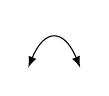
\begin{tikzpicture}
\draw[black, <->, >=latex] (-0.33, -0.5) .. controls (-0.125, 0) and (0.125, 0) .. (0.33, -0.5);
\end{tikzpicture}}

\newcommand{\CVdownInc}{%
\begin{tikzpicture}
\draw[black, ->, >=latex] (-0.5, -0.5) .. controls (-0.5, -0.3) and (-0.5, -0.1) .. (0,0);
\end{tikzpicture}}

\newcommand{\CVdownDec}{%
\begin{tikzpicture}[rotate=-90]
\draw[black, ->, >=latex] (-0.5, -0.5) .. controls (-0.5, -0.3) and (-0.5, -0.1) .. (0,0);
\end{tikzpicture}}

\begin{document}
	\noindent \hrulefill \\
	MATH-241 \hfill Pierre-Olivier Paris{\'e}\\
	Solutions Section 3-9 \hfill \semester \\\vspace*{-1cm}
	
	\noindent\hrulefill
	
	\spc
	
	\exo{2}
	\\
	The first term becomes $\tfrac{x^3}{3}$, the second term becomes $-\tfrac{3}{2} x^2$ and the last term becomes $2x$. Therefore, the most general antiderivative is
		\begin{align*}
		F(x) = \frac{x^3}{3} - \frac{3x^2}{2} + 2x + C .
		\end{align*}					

	\spc
	
	\exo{6}
	\\
	We can see that
		\begin{align*}
		f(x) = (x - 5)^2 = (x - 5)^2 \frac{d}{dx} (x - 5)
		\end{align*}
	and so from the Chain Rule, 
		\begin{align*}
		F(x) = \frac{(x - 5)^3}{3} + C .
		\end{align*}
		
	\spc
	
	\exo{12}
	\\
	We turn $\sqrt[3]{x^2}$ and $\sqrt{x}$ into exponent and then $f(x) = x^{2/3} + x x^{1/2} = x^{2/3} + x^{3/2}$. Therefore,
		\begin{align*}
		F(x) = \frac{x^{2/3 + 1}}{2/3 + 1} + \frac{x^{3/2 + 1}}{3/2 + 1} + C  = \frac{x^{5/3}}{5/3} + \frac{x^{5/2}}{5/2} + C = \frac{3}{5} x^{5/3} + \frac{2}{5} x^{5/2} + C .
		\end{align*}
	Therefore, $F(x) = \frac{3}{5} x^{5/3} + \frac{2}{5} x^{5/2} + C$.
	
	\spc
	
	\exo{14}
	\\
	We simplify $g(x)$:
		\begin{align*}
		g(x) = \frac{5}{x^6} - \frac{4}{x^3} + 2 = 5x^{-6} - 4x^{-3} + 2 .
		\end{align*}
	Therefore, we obtain
		\begin{align*}
		G(x) = \frac{5}{-6 + 1} x^{-6 + 1} - \frac{4}{-3 + 1} x^{-3 + 1} + 2x + C = \frac{5}{-5} x^{-5} - \frac{4}{-2} x^{-2} + 2x +  C .
		\end{align*}
	After simplifications, $G(x) = -x^{-5} + 2x^{-2} + 2x + C$.
	
	\spc
	
	\exo{16}
	\\
	The antiderivative of $\cos t$ is $\sin t$ because $(sin t)' = \cos t$ and the antiderivative of $\sin t$ is $-\cos (t)$ because $(-\cos t)' = - (-\sin t) = \sin t$. Therefore,
		\begin{align*}
		F(t) = 3 \sin t + 4 \cos t + C .
		\end{align*}
		
	\spc
	
	\exo{22}
	\\
	The most general antiderivative of $f(x)$ is
		\begin{align*}
		F(x) = \frac{x^2}{2} - 2 \cos x + C .
		\end{align*}
	Since $F(0) = -6$, we then have the following equation for $C$:
		\begin{align*}
		-6 = \frac{0^2}{2} - 2 \cos (0) + C \iff -6 = -2 + C \iff -4 = C .
		\end{align*}
	Therefore, the antiderivative satisfying $F(0) = -6$ is $F(x) = \tfrac{x^2}{2} - 2\cos x - 4$.
	
	\spc
	
	\exo{24}
	\\
	Let $g(x) = f'(x)$, so that $g'(x) = f''(x)$. We first find $g(x)$. We have $g'(x) = x^6 - 4x^4 + x + 1$, so that
		\begin{align*}
		g(x) = \frac{x^7}{7} - \frac{4x^5}{5} + \frac{x^2}{2} + x + C .
		\end{align*}
	We know that $f'(x) = g(x)$, so that
		\begin{align*}
		f(x) = \frac{x^8}{56} - \frac{2x^6}{15} + \frac{x^3}{6} + \frac{x^2}{2} + Cx + D .
		\end{align*}
		
	\spc
	
	\exo{33}
	\\
	We simplify the expression of $f'(x)$:
		\begin{align*}
		f'(x) = \sec^2 (t) + \sec t \tan t .
		\end{align*}
	An antiderivative for $\sec^2 (t)$ is $\tan (t)$ because $(\tan t)' = \sec^2 t$ and an antiderivative for $\sec t \tan t$ is $\sec t$ because $(\sec t)' = \sec t \tan t$. Therefore, we have
		\begin{align*}
		f(x) = \tan t + \sec t + C .
		\end{align*}
	Since $f(\pi / 4 ) = -1$, we then have the following equation for $C$:
		\begin{align*}
		-1 = \tan (\pi/4) + \sec (\pi/4) + C \iff -1 = 1 + \frac{1}{\sqrt{2}{2}} + C \iff 2 - \frac{2}{\sqrt{2}} = C .
		\end{align*}
	Therefore, $f(x) = \tan t + \sec t + 2 - \frac{2}{\sqrt{2}}$.
		
		
\end{document}